% Included inside the monitoring section in Chapter 4.
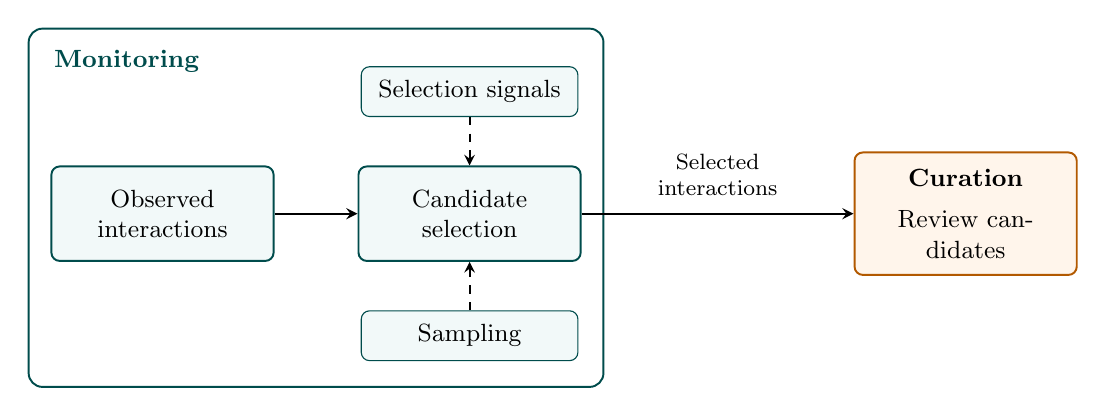
\begin{tikzpicture}[
  process/.style={
    draw, rounded corners=3pt, line width=0.7pt,
    text width=2.4cm, minimum height=1.2cm,
    inner sep=6pt, align=center, font=\small
  },
  guide/.style={
    draw=teal!60!black, rounded corners=3pt, fill=teal!5,
    text width=2.4cm, inner sep=5pt, align=center, font=\small
  },
  flow/.style={->, >=stealth, line width=0.8pt},
  influence/.style={->, >=stealth, dashed, line width=0.7pt},
  transition/.style={align=center, font=\footnotesize, fill=white, inner sep=3pt}
]
  \draw[draw=teal!60!black, rounded corners=5pt, line width=0.7pt]
    (-1.7,-2.2) rectangle (5.6,2.35);
  \node[anchor=north west, font=\small\bfseries, text=teal!60!black]
    at (-1.5,2.2) {Monitoring};

  \node[process, draw=teal!60!black, fill=teal!5] (interactions) at (0,0)
    {Observed\\interactions};
  \node[process, draw=teal!60!black, fill=teal!5] (selection) at (3.9,0)
    {Candidate\\selection};
  \node[guide] (signals) at (3.9,1.55) {Selection signals};
  \node[guide] (sampling) at (3.9,-1.55) {Sampling};
  \node[process, draw=orange!70!black, fill=orange!8] (curation) at (10.2,0)
    {\textbf{Curation}\\[4pt]Review candidates};

  \draw[flow] (interactions.east) -- (selection.west);
  \draw[influence] (signals.south) -- (selection.north);
  \draw[influence] (sampling.north) -- (selection.south);
  \draw[flow] (selection.east) -- node[transition, above=3pt]
    {Selected\\interactions} (curation.west);
\end{tikzpicture}
